%------------------------------------------------------------------------
% Presentation example for students by Markus Koschi
%
% compile with LaTeX + dvips + ps2pdf or 
% compile with PdfLaTeX after removing all eps figures 

\pdfminorversion=7

%------------------------------------------------------------------------
\documentclass[shortpres,aspectratio=43]{beamer}
%\documentclass[shortpres,aspectratio=169]{beamer}
\usetheme{CambridgeUS}

\setbeamertemplate{footline}
{
  \leavevmode%
  \hbox{%
  \begin{beamercolorbox}[wd=.333333\paperwidth,ht=2.25ex,dp=1ex,left]{author in head/foot}%
  \hspace*{4ex}\usebeamerfont{author in head/foot}\insertshortauthor%~~\beamer@ifempty{\insertshortinstitute}{}{(\insertshortinstitute)}
  \end{beamercolorbox}%
  \begin{beamercolorbox}[wd=.333333\paperwidth,ht=2.25ex,dp=1ex,center]{title in head/foot}%
    \usebeamerfont{title in head/foot}\insertshorttitle
  \end{beamercolorbox}%
  \begin{beamercolorbox}[wd=.333333\paperwidth,ht=2.25ex,dp=1ex,right]{date in head/foot}%
    %\usebeamerfont{date in head/foot}\insertshortdate{}\hspace*{2em}
    \insertframenumber{} / \inserttotalframenumber\hspace*{2ex}
  \end{beamercolorbox}}%
  \vskip0pt%
}\part{title}
\beamertemplatenavigationsymbolsempty

%color specification-----------------------------------------------------
\definecolor{TUMblue}{RGB}{27, 94, 170}%{rgb}{0.00, 0.40, 0.74}
\definecolor{TUMgray}{rgb}{0.85, 0.85, 0.86}
\definecolor{TUMpantone285C}{rgb}{0.00, 0.45, 0.81}
\definecolor{TUMpantone300C}{RGB}{27, 94, 170} %uncorrected TUMpantone300C
\definecolor{lightblue}{RGB}{213,227,241}%{rgb}{0.7529,0.8118,0.9333}

\setbeamercolor{block title}{fg=white, bg=TUMblue}
\setbeamercolor{block body}{bg=lightblue}
\setbeamertemplate{blocks}[rounded][shadow=true]

%------------------------------------------------------------------------
\setbeamercolor{frametitle}{bg=TUMblue, fg=white}
\setbeamercolor{palette primary}{bg=TUMblue, fg=white}%{fg=TUMblue,bg=TUMgray}
\setbeamercolor{palette secondary}{use=palette primary,bg=TUMblue, fg=white}
\setbeamercolor{palette tertiary}{use=palette primary,fg=white, bg=TUMblue}
\setbeamercolor{palette quaternary}{use=palette primary,fg=white, bg=TUMblue}

\setbeamercolor{title}{bg=TUMblue,fg=white}
\setbeamercolor{item projected}{use=item,fg=black,bg = lightblue}
\setbeamercolor{block title}{fg=black, bg=lightblue}
\setbeamercolor{block body}{bg=white}
\setbeamertemplate{blocks}[rounded][shadow=true]

%------------------------------------------------------------------------
\setbeamertemplate{bibliography item}{\insertbiblabel}
\setbeamercolor{bibliography item}{parent=palette primary}
\setbeamercolor{bibliography entry author}{fg=TUMblue}

% define vspace size 
\newlength{\mylength}
\setlength{\mylength}{0.1cm}

%------------------------------------------------------------------------
\usepackage{subfigure}
\usepackage{textpos} % for figure (logo) on slides
\usepackage{psfrag} % for \psfrag in figures
%\usepackage{algorithm,algpseudocode} % for algorithm environment
%\usepackage{booktabs} % for rulers in tables
\usepackage{units} % for units to values
%\usepackage{hyperref}
%\usepackage{graphicx}
\usepackage{tikz}
\usepackage{color}
\usepackage{mathtools}
\usepackage{amsmath}
\usepackage{amsfonts}
\usepackage{svg}
\usepackage{tikz}
\usepackage{pgfplots}

\usepackage{scrhack} % necessary for listings package
\usepackage{listings}
\usepackage{lstautogobble}

\usepackage{xcolor}

% Settings for lstlistings
\lstset{%
  basicstyle=\ttfamily,
  columns=fullflexible,
  autogobble,
  keywordstyle=\bfseries\color{TUMBlue},
  stringstyle=\color{TUMAccentGreen}
}

\definecolor{mGreen}{rgb}{0,0.6,0}
\definecolor{mGray}{rgb}{0.5,0.5,0.5}
\definecolor{mPurple}{rgb}{0.58,0,0.82}
\definecolor{backgroundColour}{rgb}{0.95,0.95,0.92}

\lstdefinestyle{GoStyle}{
    language=Go,
    basicstyle=\ttfamily\small,
    keywordstyle=\color{blue}\bfseries,
    commentstyle=\color{mGreen},
    stringstyle=\color{red},
    numberstyle=\tiny\color{gray},
    backgroundcolor=\color{white},
    frame=single,
    tabsize=4,
    captionpos=b,
    breaklines=true,
    breakatwhitespace=true,
    showspaces=false,
    showstringspaces=false,
    numbers=left,
    numbersep=5pt,
    morekeywords=[2]{ConnectionIdUpdateBPFHandler, localUpdateConnectionId, Bytes, Len, RetrieveNextPacketFromMap, RegisterBPFPacket}, % Add your method names here
    keywordstyle=[2]{\color{brown}\bfseries}, % Style for method names
    morekeywords=[3]{struct, interface, func, import, package, defer, go, select, case, chan, map, type, const, var, range, fallthrough, continue, break, default},
}



%-----------------------------------------------------------------------
\newcommand{\at}{\fontfamily{ptm}\selectfont @}
\newcommand{\ra}[1]{\renewcommand{\arraystretch}{#1}} %to change the row spacing in tables

\newcommand\blfootnote[1]{%
  \begingroup
  \renewcommand\thefootnote{}\footnote{#1}%
  \addtocounter{footnote}{-1}%
  \endgroup
}

%-----------------------------------------------------------------------
\title[eBPF-Assisted Relay Setup]{eBPF-Assisted Relays for Multimedia Streaming}

\author[Daniel Pfeifer]{Daniel Alexander Antonius Pfeifer}
\institute[TU M\"unchen]{Technical University of Munich}

\date\today

%---------------------------------------------------------------------
\begin{document}

%% TUM logo
\addtobeamertemplate{frametitle}{}{%
\begin{textblock*}{\textwidth}(.92\textwidth,-0.775cm) % for aspectratio=43

\includegraphics[height=0.60cm]{./figures/TUM_Logo_weiss_e.eps} % for aspectratio=43
%\begin{textblock*}{\textwidth}(.92\textwidth,-0.93cm) % for aspectratio=169
%
\includegraphics[height=0.7cm]{./figures/TUM_Logo_weiss_e.eps} % for aspectratio=169
\end{textblock*}}


\begin{frame}[plain]
    \titlepage%
\end{frame}

\begin{frame}{}
  \tableofcontents
\end{frame}


% Interesting figures:
\iffalse%
figures/02_background/adaptive-bitrate-streaming.drawio.pdf
figures/02_background/general-relay.drawio.pdf
figures/02_background/hook-point-locations.drawio.pdf

figures/03_fast_relays/forward-registration.drawio.pdf (maybe too detailed)
figures/03_fast_relays/packet-forwarding.drawio.pdf
figures/03_fast_relays/priority-streams.drawio.pdf
figures/03_fast_relays/retransmission.drawio.pdf (maybe too detailed)
figures/03_fast_relays/route-layering.drawio.pdf
figures/03_fast_relays/ebpf-setup.drawio.pdf

figures/04_testing_and_results/delays_small_packets_simple_userspace.pdf
figures/04_testing_and_results/cpu_usage_server_ns.pdf
figures/04_testing_and_results/cpu_usage_relay_ns.pdf
figures/04_testing_and_results/cpu_usage_client_ns.pdf
\fi

% ----------------------------------------------------------------------- Begin Section Introduction 

\section{Introduction}

\begin{frame}{}
  \tableofcontents[currentsection]
\end{frame}

\begin{frame}{Motivation}
    \begin{minipage}{0.3\textwidth}
        \begin{itemize}
            \item Shorten Critical Path
            \vspace{\mylength}
            \item Avoid Network Stack Traversal
            \vspace{\mylength}
            \item Reduce Forwarding Delay
        \end{itemize}
    \end{minipage}\hfill
    \begin{minipage}{0.6\textwidth}
        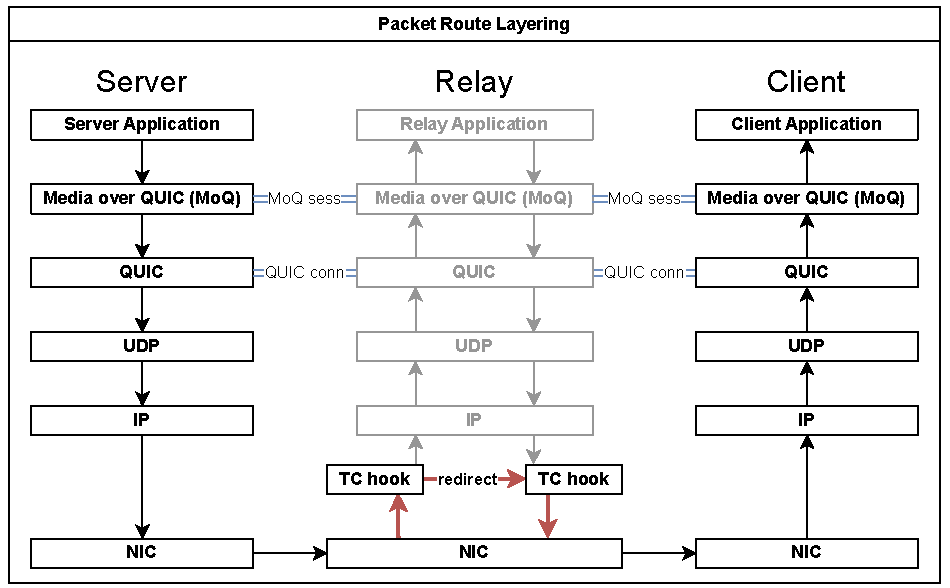
\includegraphics[
            scale=0.45
        ]{../figures/03_fast_relays/route-layering.drawio.pdf}
    \end{minipage}
\end{frame}

\begin{frame}{Research Question}
    \begin{itemize}
        \item \textit{Improve relay performance by using eBPF technology?}
        \vspace{2\mylength}
        \begin{itemize}
            \item \textit{Remove userspace packet-processing from critical path?}
            \vspace{2\mylength}
            \item \textit{Handle packet en- and decryption?}
            \vspace{2\mylength}
            \item \textit{Communication between userspace and the eBPF program?}
            \vspace{2\mylength}
            \item \textit{Generalize to support other protocols?}
        \end{itemize}
    \end{itemize}
\end{frame}

% ----------------------------------------------------------------------- Begin Section QUIC and eBPF

\section{QUIC and eBPF}

\begin{frame}{}
  \tableofcontents[currentsection]
\end{frame}

\begin{frame}{QUIC}
    \begin{minipage}{0.45\textwidth}
        \begin{itemize}
            \item Started by Google as \textit{Quick UDP Internet Connections}
            \vspace{2\mylength}
            \item Standardized by IETF
            \vspace{2\mylength}
            \item Fast Development Cycle since Userspace Implementation
            \vspace{2\mylength}
            \item Gets rid of Issues like Head-of-Line Blocking
        \end{itemize}
    \end{minipage}\hfill
    \begin{minipage}{0.53\textwidth}
        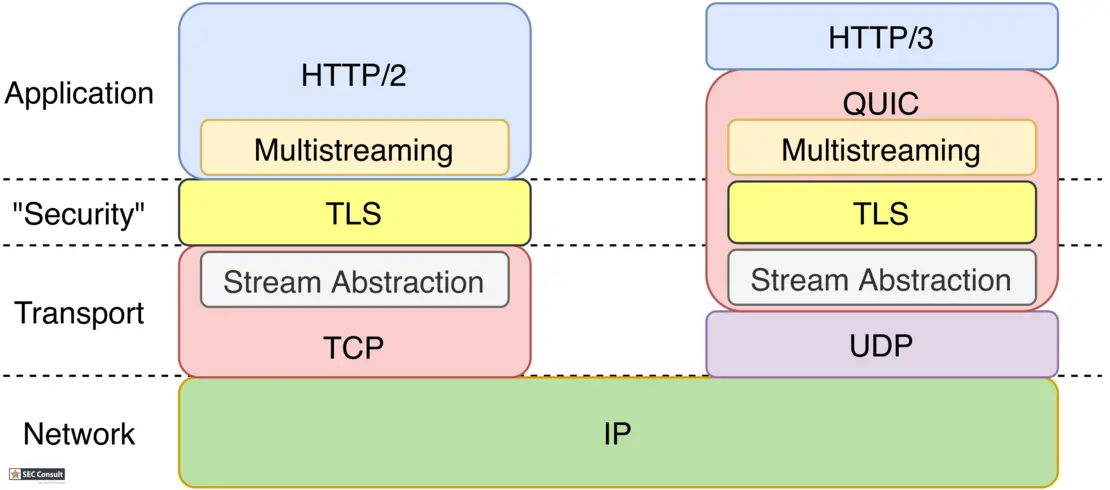
\includegraphics[
            scale=0.15
        ]{figures/quic.png}
        \Tiny{Source: https://sec-consult.com/blog/detail/better-dont-be-too-quick/} % TODO: correct citing?
    \end{minipage}
\end{frame}

\begin{frame}{eBPF}
    \begin{minipage}{0.55\textwidth}
        \begin{itemize}
            \item Kernel-Internal Virtual Machine
            \vspace{2\mylength}
            \item Used for Packet Filtering and Tracing
            \vspace{2\mylength}
            \item Multiple Hook-Points in the Kernel (e.g. XDP and TC)
            \vspace{2\mylength}
            \item Userspace Communication via Maps
        \end{itemize}
    \end{minipage}\hfill
    \begin{minipage}{0.43\textwidth}
        \centering
        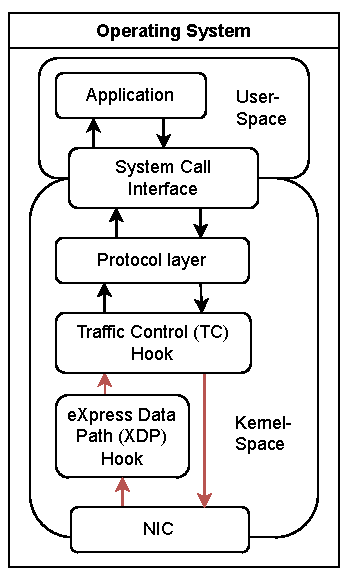
\includegraphics[
            scale=0.6
        ]{../figures/02_background/hook-point-locations.drawio.pdf}
    \end{minipage}
\end{frame}

% ----------------------------------------------------------------------- Begin Section Fast-Relays

\section{Fast-Relays}

\begin{frame}{}
  \tableofcontents[currentsection]
\end{frame}

\begin{frame}{QUIC Adaptations}
    \begin{minipage}{\textwidth}
        \begin{itemize}
            \item Turn off en- and decryption
            \vspace{2\mylength}
            \item Priorities for packets
            \vspace{2\mylength}
            \item Public endpoint for packet registration
            \vspace{2\mylength}
            \item Function pointer additions for eBPF state handling
            \vspace{2\mylength}
            \begin{itemize}
                \item Relay developer defines functions for eBPF map access
                \vspace{2\mylength}
                \item Called within quic-go if defined
            \end{itemize}
        \end{itemize}
    \end{minipage}
\end{frame}

% Packet Priorities

\begin{frame}[fragile]{Public Endpoint for Packet Registration}
    \begin{minipage}{\textwidth}
        \begin{lstlisting}[style=GoStyle,
            caption=Packet registration within relay code.]
            go func(conn quic.Connection) {
                /* ... */
                for {
                    /* ... */
                    packet := common.RetrieveNextPacketFromMap()
                    conn.RegisterBPFPacket(packet)
                    /* ... */
                }
            }(conn)
        \end{lstlisting}
    \end{minipage}
\end{frame}

% Function Pointer Additions

\begin{frame}{eBPF Setup}
    \begin{minipage}{0.43\textwidth}
        \begin{itemize}
            \item Three eBPF Programs
            \vspace{2\mylength}
            \begin{itemize}
                \item Client ingress (client registration)
                \vspace{2\mylength}
                \item Server ingress (packet duplication and forwarding)
                \vspace{2\mylength}
                \item Client egress (state management)
            \end{itemize}
        \end{itemize}
    \end{minipage}\hfill
    \begin{minipage}{0.55\textwidth}
        \centering
        \begin{figure}
            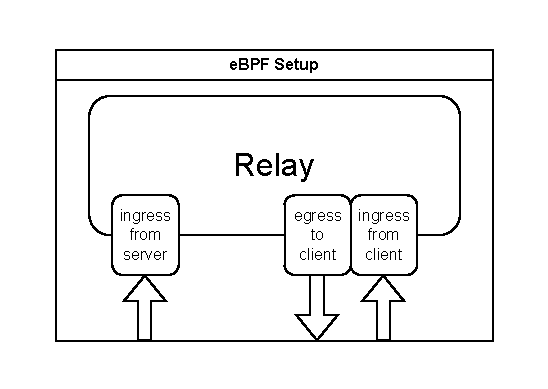
\includegraphics[scale=0.6]{../figures/03_fast_relays/ebpf-setup.drawio.pdf}
        \end{figure}
        \vspace{2\mylength}
        \begin{figure}
            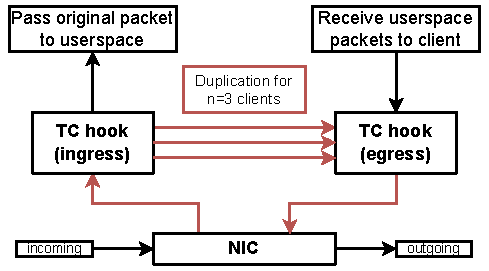
\includegraphics[scale=0.7]{../figures/03_fast_relays/packet-forwarding.drawio.pdf}
        \end{figure}
    \end{minipage}
\end{frame}

\begin{frame}{Userspace Synchronization}
    \begin{minipage}{\textwidth}
        \begin{itemize}
            \item Number of clients
            \vspace{2\mylength}
            \item Connection state (e.g.~connection-id, id-translations, etc.)
            \vspace{2\mylength}
            \item Incoming packet information (e.g.~timestamp, etc.)
            \vspace{2\mylength}
            \item Priority drop threshold for a connection
            \vspace{2\mylength}
            \item Congestion control updates
        \end{itemize}
    \end{minipage}
\end{frame}

\begin{frame}{Userspace Synchronization cont.}
    \begin{minipage}{\textwidth}
        \centering
        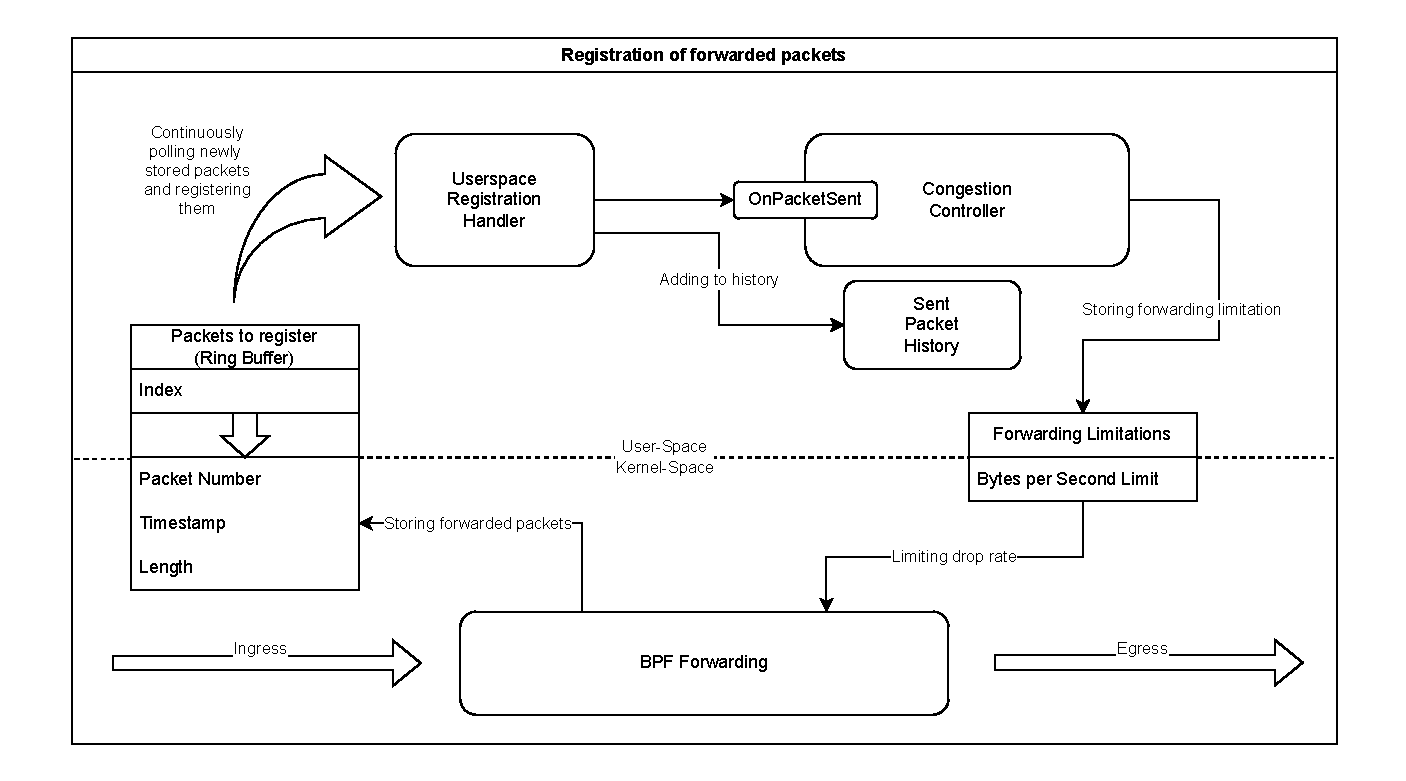
\includegraphics[scale=0.6]{../figures/03_fast_relays/forward-registration.drawio.pdf}
    \end{minipage}
\end{frame}

\iffalse%
% uint8_t client_prio_drop_limit = value->priority_drop_limit;
% uint8_t packet_prio; 
% SAVE_BPF_PROBE_READ_KERNEL(&packet_prio, sizeof(packet_prio), payload + 1 /* Short header flags */);

% if (packet_prio < client_prio_drop_limit) {
%     bpf_printk("Packet priority lower than client priority threshold!\n");
%     return TC_ACT_SHOT;
% }
\fi

% \begin{frame}{Congestion Considerations}
%    TODO
% \end{frame}

\begin{frame}{Packet Retransmission}
    \begin{minipage}{\textwidth}
        \begin{itemize}
            \item Retransmission happen at stream level
            \vspace{2\mylength}
            \item Relay might not have correct stream state
            \vspace{2\mylength}
            \item Client needs \textbf{all} parts of a frame for correct media display
        \end{itemize}
    \end{minipage}
\end{frame}

\begin{frame}{Packet Retransmission cont.}
    \begin{minipage}{\textwidth}
        \centering
        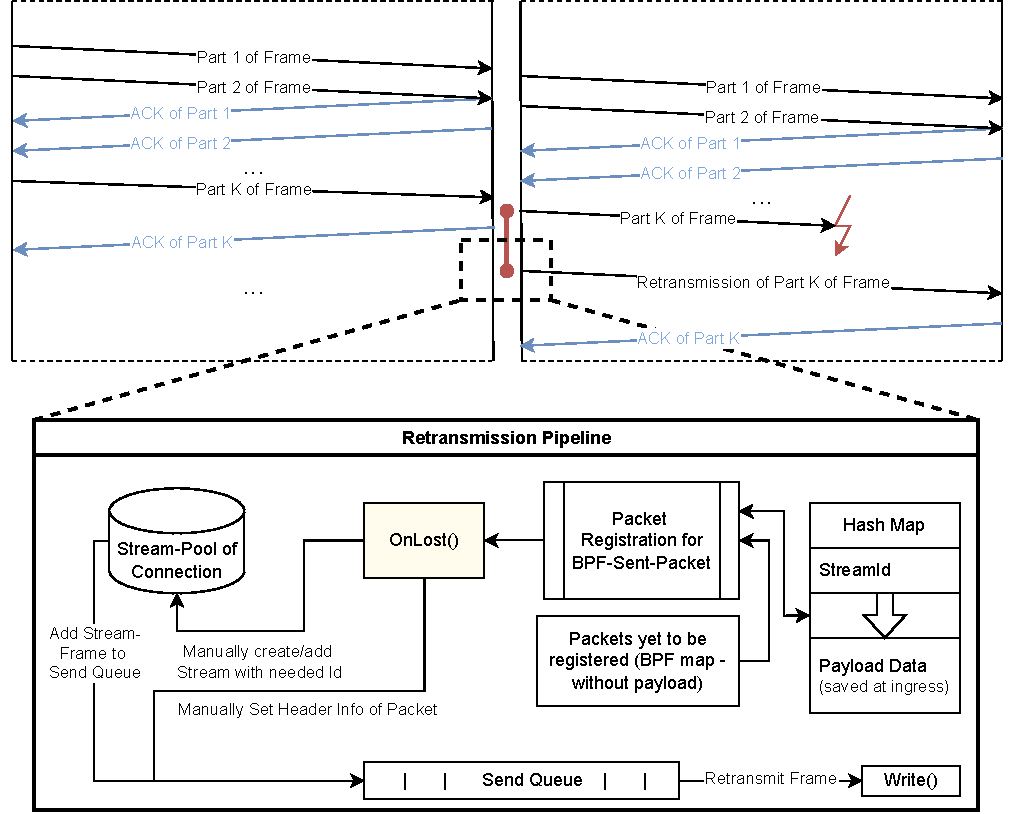
\includegraphics[scale=0.5]{figures/retransmission-presentation.drawio.pdf}
    \end{minipage}
\end{frame}

% ----------------------------------------------------------------------- Begin Section Testing

\section{Testing and Results}

\begin{frame}{}
  \tableofcontents[currentsection]
\end{frame}

\begin{frame}{Test Setup}
    \begin{minipage}{\textwidth}
        \centering
        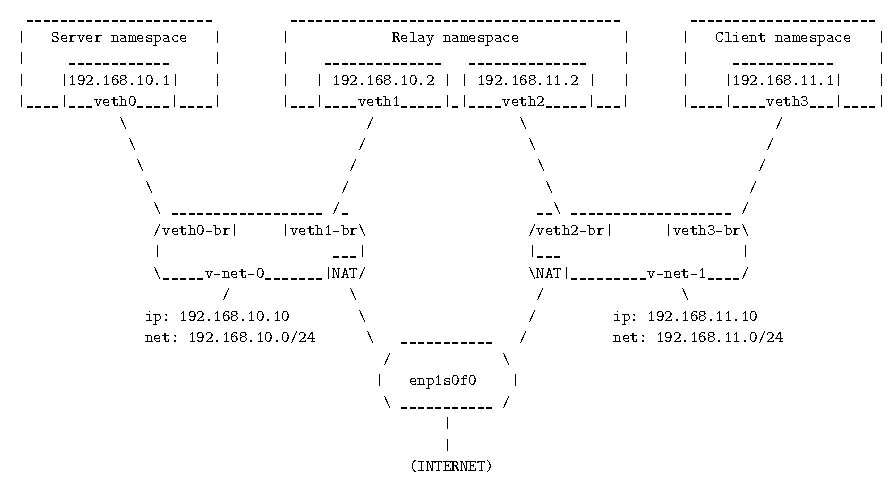
\includegraphics[scale=0.7]{figures/ns-setup.pdf}
    \end{minipage}
\end{frame}

\begin{frame}{Test Results Delay Reduction}
    \begin{minipage}{\textwidth}
        \centering
        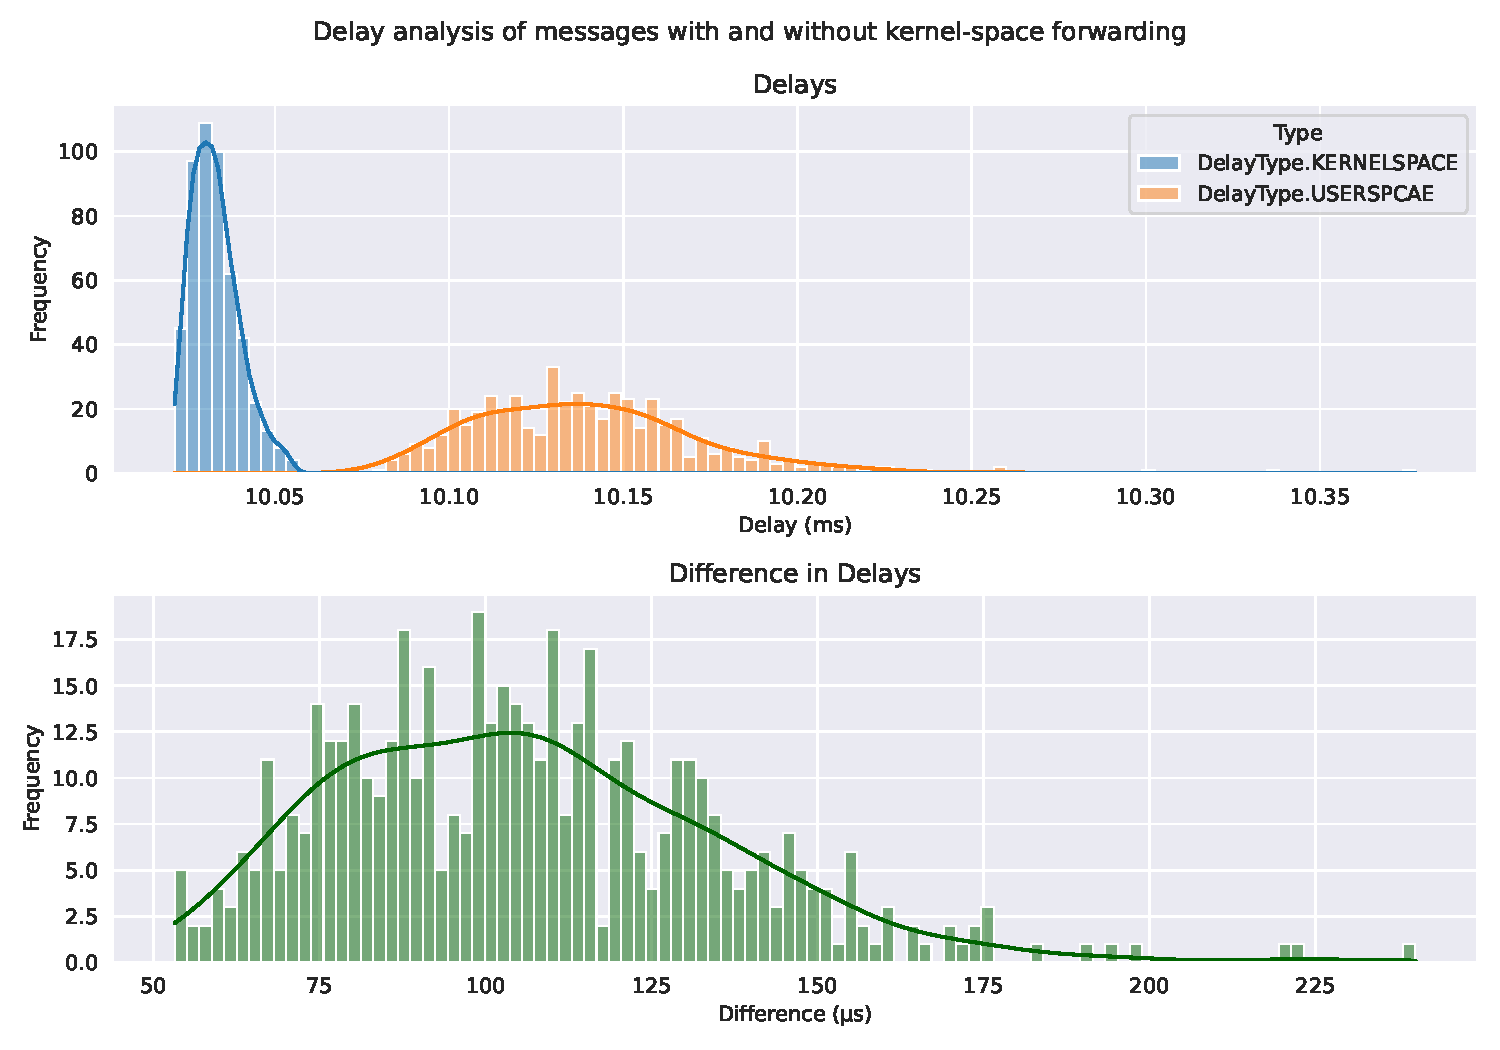
\includegraphics[scale=0.4]{../figures/04_testing_and_results/delays_small_packets_simple_userspace.pdf}
    \end{minipage}\hfill
\end{frame}

\begin{frame}{Test Results CPU Usage}
    \begin{minipage}{0.4\textwidth}
        \begin{itemize}
            \item No Impact on CPU Usage
            \vspace{2\mylength}
            \item Fewer System Calls
            \vspace{2\mylength}
            \begin{itemize}
                \item Mainly due to reduced Userspace Synchronization
            \end{itemize}
        \end{itemize}
    \end{minipage}\hfill
    \begin{minipage}{0.58\textwidth}
        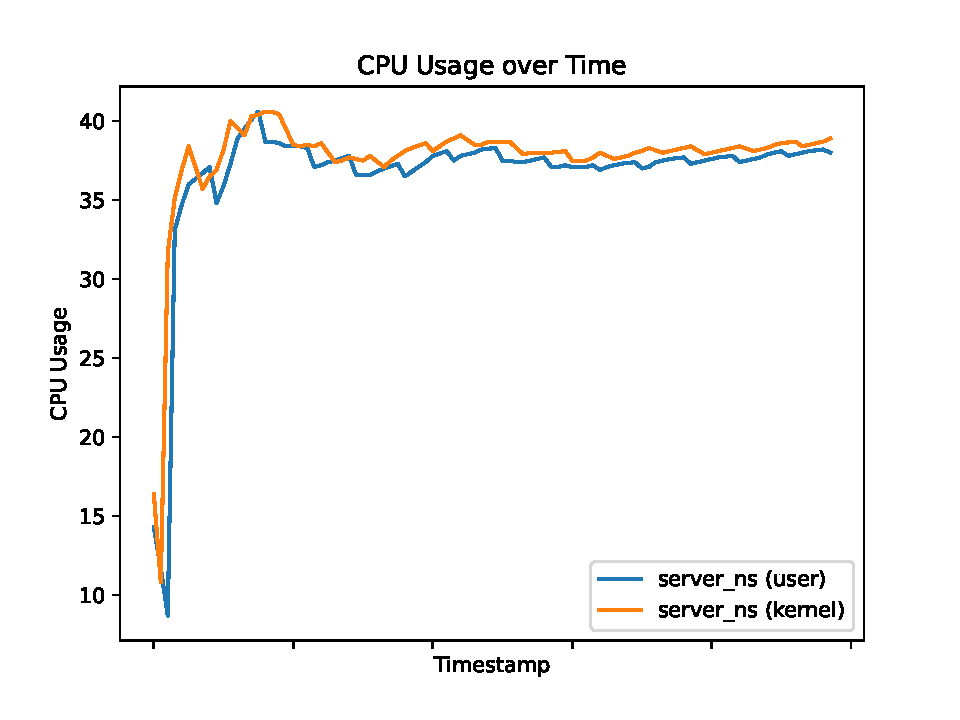
\includegraphics[scale=0.21]{../figures/04_testing_and_results/cpu_usage_server_ns.pdf}
        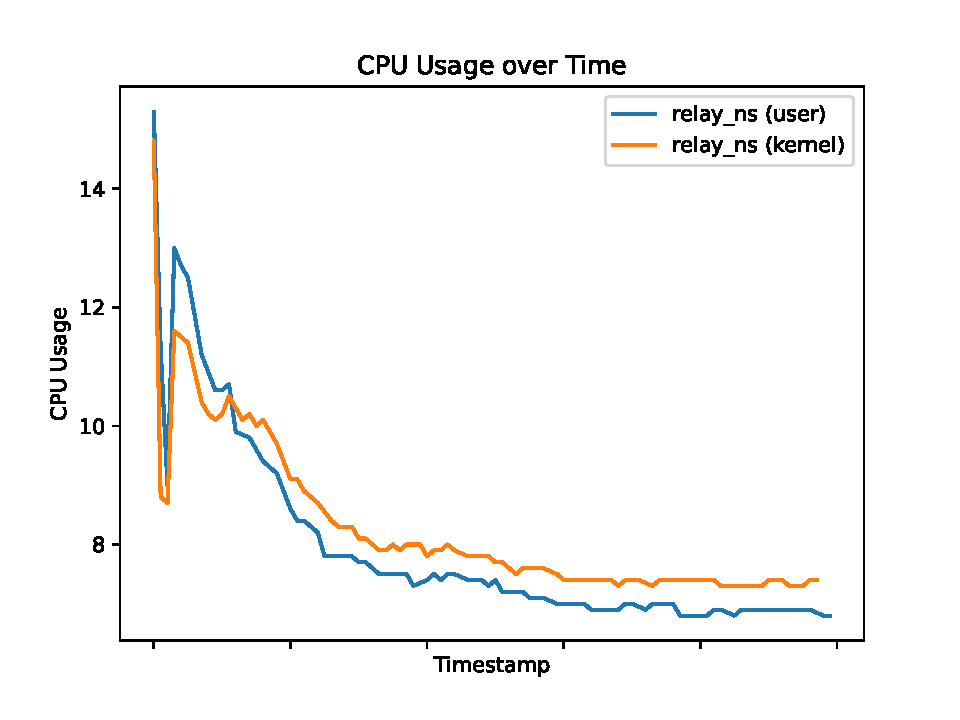
\includegraphics[scale=0.21]{../figures/04_testing_and_results/cpu_usage_relay_ns.pdf}
        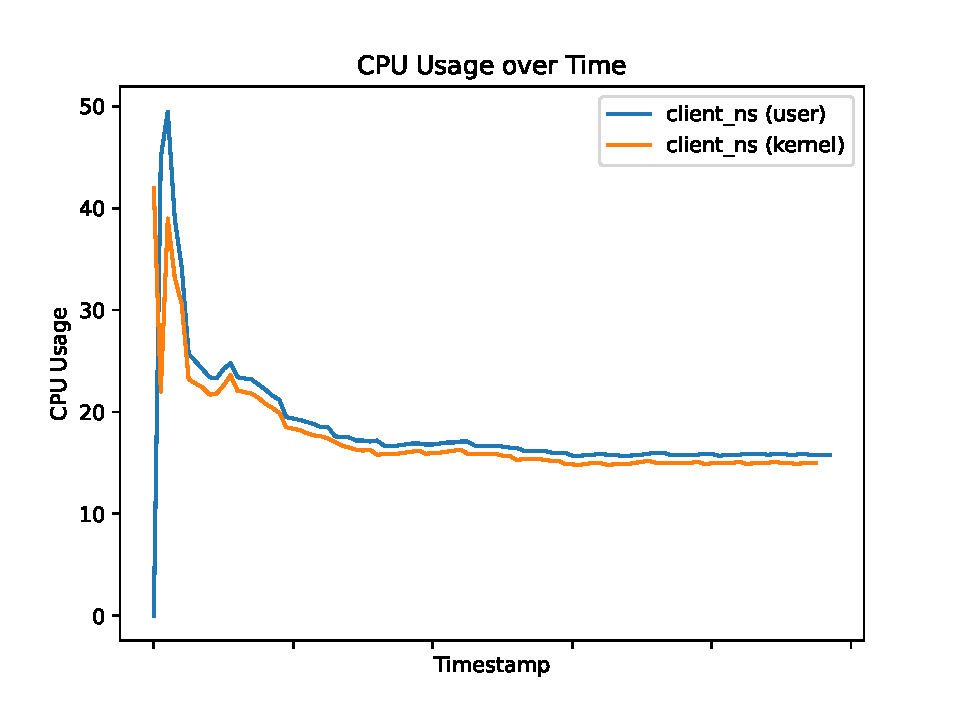
\includegraphics[scale=0.21]{../figures/04_testing_and_results/cpu_usage_client_ns.pdf}
    \end{minipage}
\end{frame}

\begin{frame}{System Calls}
    \begin{minipage}{0.43\textwidth}
        \begin{itemize}
            \item Example Stream of 30 Seconds
            \vspace{2\mylength}
            \item Overall System Calls 
            \vspace{2\mylength}
            \begin{itemize}
                \item Userspace forwarding: 296132 calls
                \vspace{2\mylength}
                \item eBPF forwarding: 225674 calls
                \vspace{2\mylength}
                \item Reduction of 24\%
            \end{itemize}
        \end{itemize}
    \end{minipage}\hfill
    \begin{minipage}{0.51\textwidth}
        \begin{itemize}
            \item \textit{futex}
            \vspace{2\mylength}
            \begin{itemize}
                \item Reduction of 34\%
                \vspace{2\mylength}
                \item 21666 calls instead of 32940
            \end{itemize}
            \vspace{2\mylength}
            % --------------------
            \item \textit{nanosleep}
            \vspace{2\mylength}
            \begin{itemize}
                \item Reduction of 42\%
                \vspace{2\mylength}
                \item 14293 calls instead of 24716
            \end{itemize}
            \vspace{2\mylength}
            % --------------------
            \item \textit{epoll\_wait}
            \vspace{2\mylength}
            \begin{itemize}
                \item Reduction of 67\%
                \vspace{2\mylength}
                \item 11289 calls instead of 34149
            \end{itemize}
            \vspace{2\mylength}
        \end{itemize}
    \end{minipage}
\end{frame}

% ----------------------------------------------------------------------- Begin Section Conclusion and Future Work

\section{Conclusion and Future Work}

\begin{frame}{}
  \tableofcontents[currentsection]
\end{frame}

\begin{frame}{Conclusion}
    \begin{itemize}
        \item Delay reduction via eBPF forwarding
        \vspace{2\mylength}
        \item More application specific relay code needed
        \vspace{2\mylength}
        \item No impact on CPU usage
    \end{itemize}
\end{frame}

\begin{frame}{Future Work}
    \begin{itemize}
        \item Hardware offloading of en- and decryption
        \vspace{2\mylength}
        \item Expand to other protocols
        \vspace{2\mylength}
        \item Prototype completion
        \vspace{2\mylength}
        \begin{itemize}
            \item Congestion control
            \vspace{2\mylength}
            \item Physical setup for testing
        \end{itemize}
    \end{itemize}
\end{frame}

\begin{frame}
    \centering
    \Huge{That's it!}
    \\
    \vspace{4\mylength}
    \huge{Any Questions?}
\end{frame}

% ----------------------------------------------------------------------- Begin Section Additional Slides

\section*{Additional Slides}

\iffalse%

    % What parts should be put here?

    % - Packet Priorities
    % - Function Pointer Additions

\fi

\begin{frame}{Packet Priorities}
    \begin{minipage}{0.43\textwidth}
        \begin{itemize}
            \item One priority per stream 
            \vspace{2\mylength}
            \item Saved in connection-id
            \vspace{2\mylength}
            \item Additional connection-id retirement constraint
        \end{itemize}
    \end{minipage}
    \begin{minipage}{0.55\textwidth}
        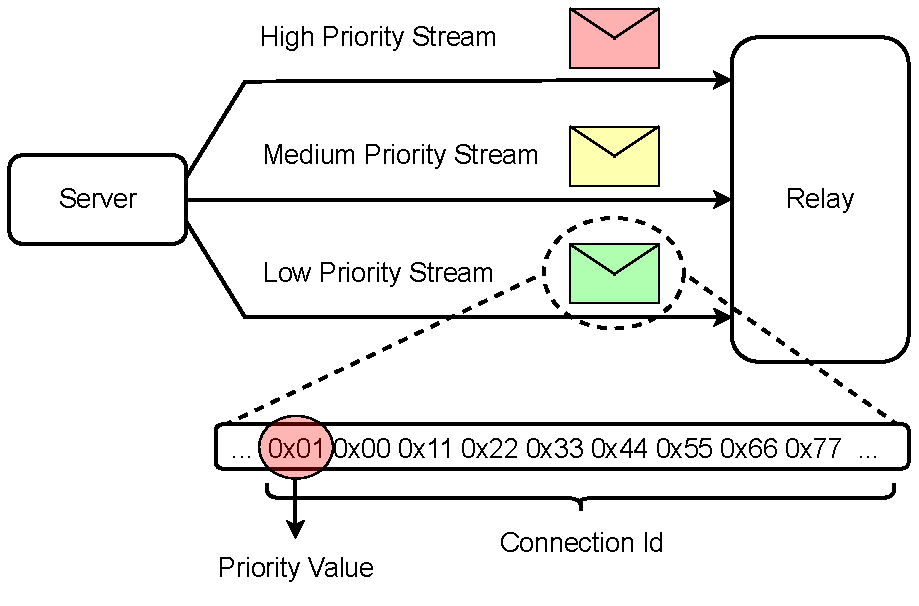
\includegraphics[scale=0.4]{../figures/03_fast_relays/priority-streams.drawio.pdf}
    \end{minipage}
\end{frame}

\begin{frame}[fragile]{Function Pointer Additions}
    \begin{minipage}{\textwidth}
        \begin{lstlisting}[style=GoStyle,
            caption=Function-pointer addition to the quic-go library.]
            /* Function pointer call within actual quic-go code */
            if packet_setting.ConnectionIdUpdateBPFHandler != nil /* && potentially other conditions */ {
                packet_setting.ConnectionIdUpdateBPFHandler(connId.Bytes(), uint8(connId.Len()), p.connection)
            }
        \end{lstlisting}
    \end{minipage}

    \begin{minipage}{\textwidth}
        \begin{lstlisting}[style=GoStyle, caption=The signature will be defined within the library itself.]
            /* Function pointer signature definition within additional config file */
            ConnectionIdUpdateBPFHandler      func(id []byte, l uint8, conn QuicConnection) = nil
        \end{lstlisting}
    \end{minipage}
\end{frame}

\begin{frame}[fragile]{Function Pointer Additions}
    \begin{minipage}{\textwidth}
        \begin{lstlisting}[style=GoStyle, label=changes:definition-function-pointer, caption=An example of how the addition looks on the relay side.]
            /* Definition of the function within the local relay code */
            func localUpdateConnectionId(id []byte, l uint8, conn packet_setting.QuicConnection) {
                /* handle the connection update by interacting with the eBPF program */
            }   

            /* Providing the function to the quic-go library */
            func main() {
                /* ... */
                packet_setting.ConnectionIdUpdateBPFHandler = localUpdateConnectionId
                /* ... */
            }
        \end{lstlisting}
    \end{minipage}
\end{frame}

\end{document}